\section{Contradiction chain}

We combine:

\begin{itemize}
\item two-time decay,
\item Carleman-weighted norms,
\item Hardy variation cost,
\item PDE curvature constraints.
\end{itemize}

Non-zero candidates generate positive weighted, variation, and curvature costs.

\begin{figure}[h]
\centering
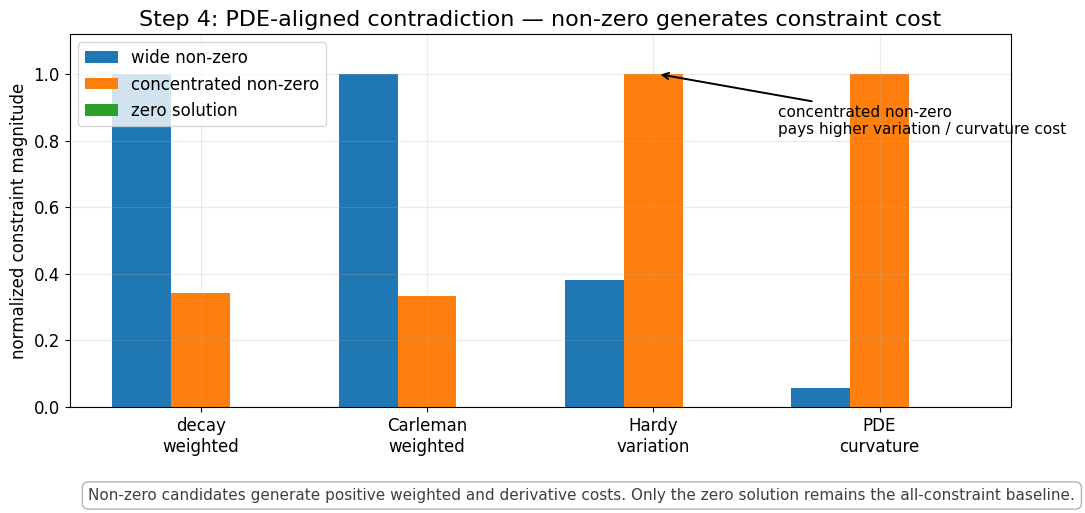
\includegraphics[width=\linewidth]{figures/step4_contradiction_pipeline_pde_code.png}
\caption{
Step 4. PDE-aligned contradiction: non-zero candidates generate incompatible constraint costs.
}
\end{figure}

\begin{figure}[h]
\centering
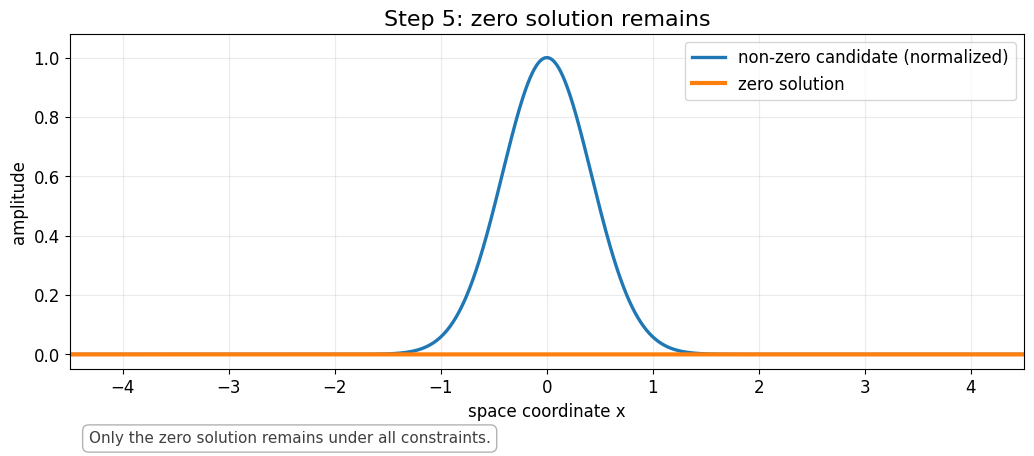
\includegraphics[width=\linewidth]{figures/step5_zero_solution_pde_code.png}
\caption{
Step 5. Zero solution: only the zero solution satisfies all constraints.
}
\end{figure}

\textbf{Conclusion.}
Only the zero solution remains.
